\part{Linear Regression}

\only<presentation>{\againframe{RecapDescriptiveStatistics}
\againframe{RecapProbabilityFundamentals}
\againframe{RecapDiscreteDistributions}

\begin{frame}[allowframebreaks,label=RecapContinousProbabilityDistributions]{Recap: Continuous Probability Distributions}
    Previously, we transitioned from counting discrete events to measuring continuous physical signals.

    \textbf{1. The Probability Density Function (PDF)}
    \begin{itemize}
        \item \textbf{Probability is Area:} $P(a \leq X \leq b) = \int_{a}^{b} f(x) \,dx$.
        \item \textbf{The \lq Exact Point\rq\ Paradox:} The probability of measuring an exact, infinitely precise value is always zero.
    \end{itemize}

    \textbf{2. The Normal Curve \& Standardisation}
    \begin{itemize}
        \item \textbf{The Bell Curve:} Symmetrical, defined entirely by mean ($\mu$) and variance ($\sigma^2$).
        \item \textbf{Z-Scores:} Unitless values ($Z = \frac{X - \mu}{\sigma}$) used to compare different systems.
        \item \textbf{The Empirical Rule:} 68\%, 95\%, and 99.7\% fall within $1\sigma$, $2\sigma$, and $3\sigma$.
    \end{itemize}

    \textbf{3. The Grand Convergence}
    \begin{itemize}
        \item At large scales, discrete models (Binomial/Poisson) approximate the continuous Normal curve.
    \end{itemize}

    \begin{alertblock}{The Transition}
        We have only modelled \textbf{single variables} in isolation. Next, we learn to measure relationships between \textbf{two variables} using Linear Regression.
    \end{alertblock}
\end{frame}

}

% Section 1: Introduction
\section{Introduction}
\begin{frame}{From Isolation to Interaction}
    Up until now, we have analysed single variables in isolation (e.g., calculating the mean lifespan of a battery or the probability of a component failing). \vspace{0.5cm}
    
    However, in real-world engineering, variables interact:
    \begin{itemize}
        \item Does an increase in operating \textbf{temperature} cause a change in output \textbf{voltage}?
        \item Can we \textit{predict} a sensor's exact voltage if we know the temperature?
        \item How do we mathematically prove that a newly manufactured batch of components meets our design specifications?
    \end{itemize}
\end{frame}

% Section 2: Correlation
\section{Correlation}

\only<article>{
    In engineering, plotting experimental data on a scatter plot is an excellent first step to see if two variables interact. However, relying purely on visual inspection is subjective. Before we invest time into building complex predictive regression models, we need a way to mathematically prove both the existence and the strength of a trend---for example, linking the thermal expansion of a material to ambient temperature, or tracking signal attenuation over a distance. This is exactly what mathematical correlation allows us to do.
}

\subsection{Pearson Correlation Coefficient}
    Before we can predict a value, we need to know if a relationship exists, and how strong it is.
\only<article>{To completely remove the subjectivity of guessing with our eyes, we use a standardised metric. Developed by Karl Pearson in the late 19th century (building upon earlier work by Sir Francis Galton), the Pearson Correlation Coefficient is the standard statistical tool used to quantify the linear dependence between two variables, condensing that relationship into a single, dimensionless number.
}



\begin{frame}{Correlation: Measuring the Relationship}
    
    \begin{block}{Definition (Pearson Correlation Coefficient, $r$)}
        Correlation measures the strength and direction of the linear relationship between two continuous variables, $X$ and $Y$. 
    \end{block}
    
    The correlation coefficient $r$ always falls between \textbf{-1} and \textbf{1}:
    \begin{itemize}
        \item $\mathbf{r = 1}$: Perfect positive linear relationship (as $X$ increases, $Y$ increases).
        \item $\mathbf{r = -1}$: Perfect negative linear relationship (as $X$ increases, $Y$ decreases).
        \item $\mathbf{r = 0}$: No linear relationship at all.
    \end{itemize}
\end{frame}

\subsubsection{Engineering Example: Temperature vs. Voltage}
\begin{frame}{Engineering Example: Temperature vs. Voltage}
    
    % Safely define the width variable to prevent handout mode errors!
    \def\boxwidth{\textwidth} 
    \mode<beamer>{\def\boxwidth{0.75\textwidth}} 
    
    \begin{minipage}{\boxwidth}
        \textbf{Scenario:} We are testing a thermistor. We measure the ambient temperature ($X$) in $^\circ$C and the resulting voltage drop ($Y$) in volts. \vspace{0.5cm}
        
        \begin{itemize}
            \item If our calculated correlation is $r = 0.92$, we have a \textbf{very strong positive correlation}.
            \item \textbf{Conclusion:} We can confidently say that as ambient temperature rises, the voltage drop reliably rises alongside it.
        \end{itemize}
    \end{minipage}%
    % The QR code safely appears ONLY during the live presentation
%    \only<beamer>{%
%    \hfill
%    \begin{minipage}{0.2\textwidth}
%        \centering
%        \qrcode[height=1.2cm]{https://www.menti.com/al2ycr7buvya} \\
%        \vspace{0.1cm}
%        \scriptsize \textbf{Scan to vote!}
%    \end{minipage}%
 %   }
\end{frame}
\subsection{Calculating the Pearson Correlation Coefficient ($r$)}
\begin{frame}{Calculating the Pearson Correlation Coefficient ($r$)}
   \only<article>{ To calculate the exact correlation coefficient by hand, we use \lq Sum of Squares\rq\ formulas. These measure the individual spread of each variable and how they vary together.}
    
    \begin{block}{\only<presentation>{1. }The Sum of Squares}
        \begin{itemize}
            \item Spread of $X$: $$S_{xx} = \sum x^2 - n\bar{x}^2$$
            \item Spread of $Y$: $$S_{yy} = \sum y^2 - n\bar{y}^2$$
            \item Covariance: $$S_{xy} = \sum xy - n\bar{x}\bar{y}$$
        \end{itemize}
    \end{block}
    
    \begin{block}{\only<presentation>{2. }The Pearson Formula}
      \only<article>{The correlation coefficient $r$ is the ratio of the covariance ($S_{xy}$) to the square root of the individual variances:}
        $$r = \frac{S_{xy}}{\sqrt{S_{xx} S_{yy}}}$$
    \end{block}
    
\only<article>{The denominator mathematically normalises the value, guaranteeing the final result is strictly bounded between -1 and 1.}
\end{frame}

\subsection{Worked Example: Pearson Correlation ($r$)}
\begin{frame}{Worked Example: Pearson Correlation ($r$)}
    
    % Safely define the width variable to prevent handout mode errors!
    \def\boxwidth{\textwidth} 
    \mode<beamer>{\def\boxwidth{0.88\textwidth}} 
    
    \begin{example}[The Scenario]
        \begin{minipage}{\boxwidth}
            An engineer tests a new thermistor, measuring ambient temperature ($X$) in $^{\circ}$C and the resulting voltage drop ($Y$) in Volts for $n = 5$ data points.
        \end{minipage}%
        % The QR code safely appears ONLY during the live presentation
        \only<beamer>{%
%
        \begin{minipage}{0.1\textwidth}
            \centering
            \qrcode[height=0.8cm]{https://www.menti.com/al2ycr7buvya} \\
            \vspace{0.1cm}
            \scriptsize \textbf{Scan to vote!}
        \end{minipage}%
        }
    \end{example}
    
    \begin{block}{The Data Table}
        \centering
        \begin{tabular}{l c c c c c}
            \hline
            \textbf{Point} & \textbf{Temp ($X$)} & \textbf{Voltage ($Y$)} & \textbf{$X^2$} & \textbf{$Y^2$} & \textbf{$XY$} \\
            \hline
            1 & 20 & 0.9 & &  &  \\
            2 & 30 & 1.2 &  &  &  \\
            3 & 40 & 1.3 &  &  &  \\
            4 & 50 & 1.4 &  &  &  \\
            5 & 60 & 1.7 &  &  &  \\
            \hline
            \textbf{SUM ($\sum$)} &  && &&  \\
            \hline
        \end{tabular}
    \end{block}
    
\end{frame}

\begin{frame}{Worked Example: Means and Sum of Squares}
    \begin{solution}{Step 1: The Data Table}
        \centering
        \begin{tabular}{l c c c c c}
            \hline
            \textbf{Point} & \textbf{Temp ($X$)} & \textbf{Voltage ($Y$)} & \textbf{$X^2$} & \textbf{$Y^2$} & \textbf{$XY$} \\
            \hline
            1 & 20 & 0.9 & 400 & 0.81 & 18.0 \\
            2 & 30 & 1.2 & 900 & 1.44 & 36.0 \\
            3 & 40 & 1.3 & 1600 & 1.69 & 52.0 \\
            4 & 50 & 1.4 & 2500 & 1.96 & 70.0 \\
            5 & 60 & 1.7 & 3600 & 2.89 & 102.0 \\
            \hline
            \textbf{SUM ($\sum$)} & \textbf{200} & \textbf{6.5} & \textbf{9000} & \textbf{8.79} & \textbf{278.0} \\
            \hline
        \end{tabular}
    \end{solution}
\end{frame}

\begin{frame}{Worked Example: Means and Sum of Squares}
    \begin{solutioncont}{Step 2: Calculate the Averages ($n=5$)}
        $$\bar{x} = 200 / 5 = 40$$
        $$\bar{y} = 6.5 / 5 = 1.3$$
    \end{solutioncont}
\end{frame}
\begin{frame}
    \begin{solutioncont}{Step 3: Calculate the Sum of Squares}
        \begin{itemize}
            \item \textbf{Spread of $X$:} 
            $$S_{xx} = \sum x^2 - n\bar{x}^2 = 9000 - 5(40)^2 = 1000$$
            
            \item \textbf{Spread of $Y$:} 
            $$S_{yy} = \sum y^2 - n\bar{y}^2 = 8.79 - 5(1.3)^2 = 0.34$$
            
            \item \textbf{Covariance:} 
            $$S_{xy} = \sum xy - n\bar{x}\bar{y} = 278 - 5(40)(1.3) = 18$$
        \end{itemize}
    \end{solutioncont}
\end{frame}

\begin{frame}{Worked Example: Calculating $r$ and Conclusion}
    \begin{solutioncont}{Step 4: The Pearson Formula}
        We plug our Sum of Squares into the correlation formula:
        $$r = \frac{S_{xy}}{\sqrt{S_{xx} S_{yy}}}$$
        
        $$r = \frac{18}{\sqrt{1000 \times 0.34}} = \frac{18}{\sqrt{340}} \approx 0.976$$
    \end{solutioncont}
    \end{frame}
    \begin{frame}
    
    \begin{solutioncont}{Step 5: Engineering Conclusion}
        Our calculated correlation is \textbf{$r = 0.976$}. 
     \only<presentation>{   \vspace{0.3cm}}
        
        Because this value is extremely close to \textbf{1}, we have mathematically proven a \textbf{very strong positive linear correlation}. As the ambient temperature rises, the voltage drop reliably and predictably increases alongside it.
    \end{solutioncont}
\end{frame}

\subsection{Interpreting the Correlation Coefficient ($r$)}
\begin{frame}{Interpreting the Correlation Coefficient ($r$)}
    \only<article>{The value of $r$ tells us two things: the \textbf{direction} and the \textbf{strength} of the linear relationship.
    
    \begin{block}{Direction}
        \begin{itemize}
            \item \textbf{Positive ($r > 0$):} As $X$ increases, $Y$ increases (e.g., Temp vs. Voltage).
            \item \textbf{Negative ($r < 0$):} As $X$ increases, $Y$ decreases (e.g., Battery \% vs. Time).
        \end{itemize}
    \end{block}
    }

    \begin{block}{Strength (Rule of Thumb)}
        \centering
        \begin{tabular}{l l}
            \hline
            \textbf{Absolute Value $|r|$} & \textbf{Strength of Linear Relationship} \\
            \hline
            $0.90$ to $1.00$ & \textbf{Very Strong} (Ideal for calibration) \\
            $0.70$ to $0.90$ & \textbf{Strong} (Clear trend) \\
            $0.50$ to $0.70$ & \textbf{Moderate} \\
            $0.30$ to $0.50$ & \textbf{Weak} \\
            $0.00$ to $0.30$ & \textbf{Negligible / None} \\
            \hline
        \end{tabular}
    \end{block}

    \begin{block}{The Golden Rule}
        \only<presentation>{\centering}
        \textbf{Correlation does not imply Causation!} \only<presentation>{\\
        \small }Just because two signals are mathematically linked doesn't mean one causes the other.
    \end{block}
\end{frame}

\subsection{Correlation vs. Causation: The Classic Trap}
\begin{frame}[allowframebreaks]{Correlation vs. Causation: The Classic Trap}
    \begin{block}{The \lq Storks and Babies\rq\ Paradox}
        Historical data from several European countries shows a \textbf{strong positive correlation} between the number of storks nesting in a town and the number of human babies born there.
    \end{block}

    \begin{alertblock}{The False Conclusion}
        Based strictly on the math ($r \approx 0.8$), one might conclude that storks deliver babies, or that babies attract storks.
    \end{alertblock}

    \begin{block}{The Reality: The \lq Lurking Variable\rq }
        Neither causes the other. Both are driven by a hidden third variable: \textbf{Town Size / Rural Environment}.
        \begin{itemize}
            \item Larger rural towns have more houses (more chimneys for storks to nest on).
            \item Larger towns have more people (resulting in more babies being born).
        \end{itemize}
    \end{block}
\end{frame}



% Section 3: Regression

\section{Simple Linear Regression}
\subsection{Introduction}
\begin{frame}{Simple Linear Regression}
    Correlation tells us if a relationship exists, but \textbf{Regression} gives us the mathematical equation to actually make predictions.
    
    \begin{block}{The Line of Best Fit}
        We want to find the straight line that minimises the total error between our predictions and the actual data. The equation is:
        $$\hat{y} = mx + c$$
        \begin{itemize}
            \item \textbf{$\hat{y}$}: The predicted output (e.g., Voltage).
            \item \textbf{$x$}: The known input (e.g., Temperature).
            \item \textbf{$m$}: The gradient or slope (Engineering \textit{Sensitivity}).
            \item \textbf{$c$}: The y-intercept (Engineering \textit{Zero-Offset Error}).
        \end{itemize}
    \end{block}
\end{frame}

\subsection{The Least-Squares Method}
\begin{frame}{The Least-Squares Method}
    To find the perfect slope and intercept by hand, we reuse the exact same \lq Sum of Squares\rq\ variables we calculated for the correlation coefficient.
    
    \begin{block}{Step 1: Calculate the Gradient ($m$)}
        The slope is simply the ratio of the covariance to the spread of $X$:
        $$m = \frac{S_{xy}}{S_{xx}}$$
    \end{block}
    
    \begin{block}{Step 2: Calculate the Intercept ($c$)}
        A fundamental rule of regression is that the line of best fit \textbf{must} pass perfectly through the average of the data ($\bar{x}, \bar{y}$). We rearrange the line equation to find $c$:
        $$c = \bar{y} - m\bar{x}$$
    \end{block}
\end{frame}

\subsection{Worked Example: Thermistor Regression}
\begin{frame}{Worked Example: Thermistor Regression (Part 1)}
    \begin{block}{The Scenario}
        Let's build the prediction model for our thermistor. We already calculated the following summary statistics from our $n=5$ data points:
        \begin{itemize}
            \item Averages: $\bar{x} = 40^{\circ}\text{C}$, \hspace{0.5cm} $\bar{y} = 1.3\text{V}$
            \item Spread of Temp: $S_{xx} = 1000$
            \item Covariance: $S_{xy} = 18$
        \end{itemize}
    \end{block}

    \begin{block}{Calculating the Gradient ($m$)}
        $$m = \frac{S_{xy}}{S_{xx}} = \frac{18}{1000} = 0.018$$
    \end{block}
\end{frame}

\begin{frame}{Worked Example: Cont}
    \begin{block}{Calculating the Intercept ($c$)}
        Now we plug our slope ($m=0.018$) and our averages into the intercept formula:
        $$c = \bar{y} - m\bar{x}$$
        $$c = 1.3 - (0.018 \times 40)$$
        $$c = 1.3 - 0.72 = 0.58$$
    \end{block}

    \begin{block}{The Final Engineering Model}
        Our final prediction equation is:
        $$\hat{y} = 0.018x + 0.58$$
        \textbf{Interpretation:} The sensor has a baseline reading of 0.58V at $0^{\circ}\text{C}$, and the voltage increases by 18 mV for every $1^{\circ}\text{C}$ increase in temperature.
    \end{block}
\end{frame}

\subsection{Complete Linear Regression Example}
\begin{frame}{Complete Linear Regression Example}
    \begin{example}[Load Cell Calibration]
        An engineer calibrates a load cell by placing 10 known masses ($X$, kg) on the sensor and measuring the output voltage ($Y$, mV). Calculate the linear regression model $\hat{y} = mx + c$.
        
        \vspace{0.2cm}
        \centering
        \resizebox{\textwidth}{!}{% Scales table to fit slide width
        \begin{tabular}{c|cccccccccc|c}
            \hline
            \textbf{$X$} & 1 & 2 & 3 & 4 & 5 & 6 & 7 & 8 & 9 & 10 & $\sum x = $ \\
            \textbf{$Y$} & 3 & 5 & 4 & 7 & 6 & 8 & 9 & 11 & 10 & 12 & $\sum y = $ \\
            \hline
            \textbf{$X^2$} &  &  &  &  &  &  &  &  &  &  & $\sum x^2 = $ \\
            \textbf{$XY$} &  &  &  &  &  &  &  &  & &  & $\sum xy = $ \\
            \hline
        \end{tabular}}
    \end{example}

    % Safely displays the QR code at the bottom of the slide ONLY on the projector
    \only<beamer>{
        \vspace{0.2cm}
        \begin{center}
            \qrcode[height=1.2cm]{https://www.menti.com/al2ycr7buvya} \\
            \vspace{0.1cm}
            \scriptsize \textbf{Scan to vote!}
        \end{center}
    }
\end{frame}
    
 
\begin{frame}{Full Linear Regression Example (continued)}
\begin{solution}
        \textbf{Step 1: Fill in the table}
          \begin{tabular}{c|cccccccccc|c}
            \hline
            \textbf{$X$} & 1 & 2 & 3 & 4 & 5 & 6 & 7 & 8 & 9 & 10 & $\sum x = \mathbf{55}$ \\
            \textbf{$Y$} & 3 & 5 & 4 & 7 & 6 & 8 & 9 & 11 & 10 & 12 & $\sum y = \mathbf{75}$ \\
            \hline
            \textbf{$X^2$} & 1 & 4 & 9 & 16 & 25 & 36 & 49 & 64 & 81 & 100 & $\sum x^2 = \mathbf{385}$ \\
            \textbf{$XY$} & 3 & 10 & 12 & 28 & 30 & 48 & 63 & 88 & 90 & 120 & $\sum xy = \mathbf{492}$ \\
            \hline
        \end{tabular}
        \end{solution}

\end{frame}


\begin{frame}{Full Linear Regression Example (continued)}
   \begin{solutioncont}
        \textbf{Step 2: Calculate the Averages ($n=10$)}
        $$\bar{x} = \frac{55}{10} = 5.5 \hspace{2cm} \bar{y} = \frac{75}{10} = 7.5$$
    \end{solutioncont}
\end{frame}

\begin{frame}[plain]{Example (continued)}
    \begin{solutioncont}
        \textbf{Step 3: Calculate the Sum of Squares}
        Using our sums and averages, we calculate the variance of $X$ ($S_{xx}$) and the covariance ($S_{xy}$).

        \textbf{Spread of Mass ($S_{xx}$):}
        $$S_{xx} = \sum x^2 - n\bar{x}^2$$
        $$S_{xx} = 385 - 10(5.5)^2$$
        $$S_{xx} = 385 - 302.5 = 82.5$$
        
        \textbf{Covariance ($S_{xy}$):}
        $$S_{xy} = \sum xy - n\bar{x}\bar{y}$$
        $$S_{xy} = 492 - 10(5.5)(7.5)$$
        $$S_{xy} = 492 - 412.5 = 79.5$$
    \end{solutioncont}
\end{frame}

\begin{frame}[plain]{Example (continued)}
    \begin{solutioncont}
        \textbf{Step 4: Calculate Gradient ($m$) and Intercept ($c$)}
        $$m = \frac{S_{xy}}{S_{xx}} = \frac{79.5}{82.5} \approx 0.964$$
        $$c = \bar{y} - m\bar{x} = 7.5 - \left(\frac{79.5}{82.5}\right)(5.5) = 7.5 - 5.3 = 2.2$$
       
        \textbf{Step 5: Final Engineering Model}
        Our calculated linear regression equation is:
        $$\hat{y} = 0.964x + 2.2$$
        
        \textbf{Interpretation:} 
        \begin{itemize}
            \item \textbf{Sensitivity ($m$):} For every 1 kg added, the sensor output increases by $\approx 0.964$ mV.
            \item \textbf{Zero-Offset ($c$):} Even at 0 kg, the sensor has a baseline noise of $2.2$ mV.
        \end{itemize}
    \end{solutioncont}
\end{frame}

\begin{frame}{Full Linear Regression Example: The Plot}
    \begin{solutioncont}
        \centering
        \begin{tikzpicture}
            \begin{axis}[
                width=0.9\textwidth,
                height=0.65\textheight,
                xlabel={Mass, $X$ (kg)},
                ylabel={Voltage, $Y$ (mV)},
                xmin=0, xmax=11,
                ymin=0, ymax=14,
                grid=both,
                grid style={dashed, gray!30},
                legend pos=north west,
                legend style={font=\small, nodes={scale=0.9, transform shape}}
            ]
            
            % Plot the raw experimental data
            \addplot[
                only marks,
                mark=*,
                color=blue,
                mark size=2.5pt
            ] coordinates {
                (1,3) (2,5) (3,4) (4,7) (5,6) 
                (6,8) (7,9) (8,11) (9,10) (10,12)
            };
            \addlegendentry{Experimental Data}
            
            % Plot the calculated line of best fit
            \addplot[
                domain=0:11,
                samples=2, % Only need 2 points to draw a straight line
                color=red,
                very thick
            ] {0.9636*x + 2.2};
            \addlegendentry{Linear Fit: $\hat{y} = 0.964x + 2.2$}
            
            \end{axis}
        \end{tikzpicture}
    \end{solutioncont}
\end{frame}

\subsection{Measuring the \lq Goodness of Fit\rq\ ($R^2$)}
\begin{frame}{Measuring the \lq Goodness of Fit\rq\ ($R^2$)}
    \begin{block}{The Coefficient of Determination}
        The \textbf{Coefficient of Determination ($R^2$)} tells us exactly how much of the variation in our output is explained by our model.
        $$R^2 = r^2$$
    \end{block}

    \begin{block}{Example: Load Cell Calibration}
     \only<article>{   Using our previous sums, we calculate the Spread of $Y$ ($S_{yy} = 82.5$), which gives us our correlation ($r$):}
        $$r = \frac{S_{xy}}{\sqrt{S_{xx}S_{yy}}} = \frac{79.5}{82.5} \approx 0.964$$
        
      \only<article>{  Squaring this gives our Coefficient of Determination:}
        $$R^2 = (0.964)^2 \approx 0.929$$
    \end{block}

    \begin{alertblock}{Engineering Interpretation}
        This means \textbf{92.9\%} of the voltage change is directly explained by the mass added to the sensor. The remaining \textbf{7.1\%} is random noise or measurement error.
    \end{alertblock}
\end{frame}

\subsection{$r$ vs. $R^2$: Why the Notation Change?}
\begin{frame}{$r$ vs. $R^2$: Why the Notation Change?}
    \begin{block}{Lowercase $r$: Simple Bivariate}
       \only<article>{Used specifically for \textbf{Simple Linear Correlation}.} It measures the mathematical \lq raw connection\rq\ between exactly two variables (one $X$ and one $Y$).
    \end{block}

    \begin{block}{Uppercase $R^2$: Multiple / Predictive}
      \only<article>{  Used for \textbf{Multiple Regression}. }In real engineering, an output ($Y$) is often driven by many inputs ($X_1, X_2, X_3$). Uppercase $R^2$ represents how well the \textit{entire model} explains the outcome.
    \end{block}

    \begin{alertblock}{The Engineering Identity}
        In Simple Linear Regression \only<article>{(what we are studying now), the math perfectly collapses down, meaning:}
        $$R^2 = (r)^2$$
        \only<article>{We use uppercase $R^2$ even for simple models to stay consistent with the professional predictive software (like MATLAB or Python) used in industry.}
    \end{alertblock}
\end{frame}


\begin{frame}{What does \lq Least Squares\rq\ actually mean?}
    \begin{block}{The Residuals (The Error)}
       \only<article>{When we plot our line of best fit through the experimental data, almost none of the points touch the line perfectly. }
        The vertical distance between an actual data point and our predicted line is called a \textbf{Residual}.
    \end{block}

    \begin{block}{Why \lq Squares\rq ?}
        Some points are above the line (positive error), and some are below (negative error)\only<article>{. If we just added them up, they would cancel each other out.
        
        To fix this, } \only<presentation>{ hence } we mathematically \textbf{square} every residual \only<article>{(which makes them all positive)}. You can visualise this as drawing a literal physical square attached to every data point.
    \end{block}

    \begin{alertblock}{The Least-Squares Goal}
        The math we just did ($S_{xx}$ and $S_{xy}$) calculates the exact slope and intercept that results in the smallest possible total area of all those squares combined.
    \end{alertblock}
\end{frame}

\begin{frame}{Visualising \lq Least Squares\rq\ }
        \centering
        \begin{tikzpicture}
            \begin{axis}[
                width=0.9\textwidth,
                height=0.65\textheight,
                xlabel={Mass, $X$ (kg)},
                ylabel={Voltage, $Y$ (mV)},
                xmin=0, xmax=11,
                ymin=0, ymax=14,
                grid=both,
                grid style={dashed, gray!30},
                legend pos=north west,
                legend style={font=\small, nodes={scale=0.9, transform shape}}
            ]
            
            % Draw the geometric "Squares" of the residuals in the background
            % Calculated as: (X, Y) rectangle (X + error, Y_predicted)
            \draw[fill=orange!40, draw=orange!80, fill opacity=0.5] (1,3) rectangle (0.836, 3.164);
            \draw[fill=orange!40, draw=orange!80, fill opacity=0.5] (2,5) rectangle (2.873, 4.127);
            \draw[fill=orange!40, draw=orange!80, fill opacity=0.5] (3,4) rectangle (1.909, 5.091);
            \draw[fill=orange!40, draw=orange!80, fill opacity=0.5] (4,7) rectangle (4.946, 6.054);
            \draw[fill=orange!40, draw=orange!80, fill opacity=0.5] (5,6) rectangle (3.982, 7.018);
            \draw[fill=orange!40, draw=orange!80, fill opacity=0.5] (6,8) rectangle (6.018, 7.982);
            \draw[fill=orange!40, draw=orange!80, fill opacity=0.5] (7,9) rectangle (7.055, 8.945);
            \draw[fill=orange!40, draw=orange!80, fill opacity=0.5] (8,11) rectangle (9.091, 9.909);
            \draw[fill=orange!40, draw=orange!80, fill opacity=0.5] (9,10) rectangle (8.128, 10.872);
            \draw[fill=orange!40, draw=orange!80, fill opacity=0.5] (10,12) rectangle (10.164, 11.836);

            % Plot the raw experimental data ON TOP of the squares
            \addplot[
                only marks,
                mark=*,
                color=blue,
                mark size=2.5pt
            ] coordinates {
                (1,3) (2,5) (3,4) (4,7) (5,6) 
                (6,8) (7,9) (8,11) (9,10) (10,12)
            };
            \addlegendentry{Experimental Data}
            
            % Plot the calculated line of best fit
            \addplot[
                domain=0:11,
                samples=2, % Only need 2 points to draw a straight line
                color=red,
                very thick
            ] {0.9636*x + 2.2};
            \addlegendentry{Linear Fit: $\hat{y} = 0.964x + 2.2$}

            % Add a manual legend entry for the squares
            \addlegendimage{area legend, fill=orange!40, draw=orange!80, fill opacity=0.5}
            \addlegendentry{Squared Residuals}
            
            \end{axis}
        \end{tikzpicture}
\end{frame}

\subsection{Engineering Example: Sensor Calibration}
\begin{frame}{Engineering Example: Sensor Calibration}
    Once we have the fit we can use it to predict values. 
    \begin{example}
        After running a regression analysis on our thermistor data, we get the following equation:
        \[ V = 0.5 + 0.02 T \]
        
        \textbf{Question:} If a system is operating at \textbf{85$^\circ$C}, what voltage drop should the safety engineer expect?
    \end{example}

    % Safely displays the QR code at the bottom of the slide ONLY on the projector
    \only<beamer>{
        \vspace{0.2cm}
        \begin{center}
            \qrcode[height=1.2cm]{https://www.menti.com/al2ycr7buvya} \\
            \vspace{0.1cm}
            \scriptsize \textbf{Scan to vote!}
        \end{center}
    }
\end{frame}
    
    
    \begin{frame}
    \begin{solution}
    \[ V = 0.5 + 0.02(85) = 0.5 + 1.7 = \mathbf{2.2 \text{ volts}} \]
    
    \end{solution}
    
    \textit{Note: This allows microcontrollers to translate raw voltage back into temperature readings automatically!}
\end{frame}

\section{Beyond Linear Regression: Non-Linearity}
\subsection{Introduction}
\begin{frame}{Beyond Linear Regression: Non-Linearity}
    \begin{block}{The Engineering Reality}
        Many physical systems are \textbf{intrinsically non-linear} (e.g., cooling, radioactive decay, or stress-strain). A straight line $\hat{y} = mx + c$ in \lq raw space\rq\ would result in a very poor fit and a low $r$ value.
    \end{block}
\subsection{Lets Map}
    \begin{block}{The Mapping Strategy}
        Instead of using complex non-linear solvers, we can often \textbf{\lq map\rq} our data into a linear space. 
        \begin{enumerate}
            \item Identify the physical law (Exponential, Power, etc.).
            \item Apply a mathematical transformation (usually $\ln$ or $1/x$).
            \item Perform standard Linear Regression on the \textbf{transformed} data.
        \end{enumerate}
    \end{block}
\end{frame}

\subsubsection{Case 1: The Exponential Model}
\begin{frame}{Case 1: The Exponential Model}
    \begin{example}[Newton's Law of Cooling / Growth]
        Consider the model: $y = ae^{bx}$
    \end{example}

    \begin{solution}
        We map this to linear space by taking the natural log ($\ln$) of both sides:
        $$\ln(y) = \ln(a \cdot e^{bx})$$
        $$\ln(y) = \ln(a) + bx$$
        
       \only<presentation>{ \vspace{0.2cm}}
        \textbf{The Linear Mapping:}
        \begin{itemize}
            \item New \lq Y\rq\ variable = $\ln(y)$
            \item New \lq X\rq\ variable = $x$ (remains same)
            \item The \textbf{Gradient} ($m$) of your fit is the growth constant $b$.
            \item The \textbf{Intercept} ($c$) is $\ln(a)$.
        \end{itemize}
    \end{solution}
\end{frame}

\subsubsection{Case 2: The Power Law Model}
\begin{frame}{Case 2: The Power Law Model}
    \begin{example}[Structural Scaling / Fluid Dynamics]
        Consider the model: $y = ax^b$
    \end{example}

    \begin{solution}
        We map this using a \textbf{Log-Log transformation}:
        $$\ln(y) = \ln(ax^b)$$
        $$\ln(y) = \ln(a) + b \ln(x)$$
        
        \vspace{0.2cm}
        \textbf{The Linear Mapping:}
        \begin{itemize}
            \item New \lq Y\rq\ variable = $\ln(y)$
            \item New \lq X\rq\ variable = $\ln(x)$
            \item The \textbf{Gradient} ($m$) is the exponent $b$.
            \item The \textbf{Intercept} ($c$) is $\ln(a)$.
        \end{itemize}
    \end{solution}
\end{frame}

\begin{frame}{Summary of Linearisation Mappings}
    \begin{block}{Reference Table for Engineers}
        \centering
        \small
        \begin{tabular}{l l l l}
            \hline
            \textbf{Model} & \textbf{Equation} & \textbf{Map $X$ to...} & \textbf{Map $Y$ to...} \\
            \hline
            \textbf{Linear} & $y = mx+c$ & $x$ & $y$ \\
            \textbf{Exponential} & $y = ae^{bx}$ & $x$ & $\ln(y)$ \\
            \textbf{Power} & $y = ax^b$ & $\ln(x)$ & $\ln(y)$ \\
            \textbf{Reciprocal} & $y = a + b/x$ & $1/x$ & $y$ \\
            \textbf{Saturation} & $y = \frac{ax}{b+x}$ & $1/x$ & $1/y$ \\
            \hline
        \end{tabular}
    \end{block}

    \begin{alertblock}{The Engineering Workflow}
        To use these:
        \begin{enumerate}
            \item Transform your raw data table columns.
            \item Calculate $S_{xx}$ and $S_{xy}$ using the \textbf{transformed} values.
            \item Find $m$ and $c$, then \lq un-map\rq\ to find your physical constants.
        \end{enumerate}
    \end{alertblock}
\end{frame}

\subsection{Full Non-Linear Regression (NLLS)}
\begin{frame}{Full Non-Linear Regression (NLLS)}
    \begin{block}{What is \lq True\rq\ Non-Linear Regression?}
        \only<article>{Instead of mapping data to fit a straight line, }\textbf{Non-Linear Least Squares (NLLS)} fits a curved model directly to the raw data. There is no closed-form solution ($S_{xx}$)\only<article>{; instead, a computer uses iterative calculus.}
    \end{block}

    \begin{block}{The Gold Standard: Levenberg-Marquardt}
        \only<article>{The standard algorithm (used in MATLAB/Python) is \textbf{Levenberg-Marquardt}. }It starts with an \lq Initial Guess\rq\ and nudges the curve thousands of times to minimise the sum of squared residuals.
    \end{block}

    \begin{alertblock}{Why use this instead of Mapping?}
        \textbf{The Error Bias Trap:} Linearising data \only<article>{(like using $\ln(y)$) warps your residuals. It }\lq stretches\rq\ errors at low values and \lq squashes\rq\ them at high values. 
        
        \only<article>{NLLS treats sensor noise ($\pm 0.1$V) exactly the same across the entire range, making it the required method for high-precision aerospace and medical systems.}
    \end{alertblock}

    \begin{itemize}
        \item \textbf{Mapping:} Best for hand-calcs and understanding trends.
        \item \textbf{NLLS:} Best for precision engineering and software models.
    \end{itemize}
\end{frame}

\section{Now to Python}
\begin{frame}[fragile]
\only<article>{Engineers rarely calculate regressions by hand. Instead, we use powerful libraries like \texttt{SciPy} in Python to instantly compute the line of best fit, correlation, and residuals.}





    \insertcode{Load Cell Example in Python}{code/load_cell_regression.py}


\end{frame}

\only<article>{
    \subsubsection*{Python Function Breakdown: \texttt{scipy.stats.linregress}}
    
    When we pass our two arrays into the \texttt{linregress(x, y)} function, it calculates the least-squares regression and returns an object containing five highly useful statistical values. In our code, we \lq unpack\rq these values into five separate variables:
    
    \begin{description}
        \item[\texttt{slope}:] The gradient of the regression line ($m$). In engineering, this represents the \textbf{sensitivity} of the system (e.g., how much the voltage changes per kilogram of mass added).
        
        \item[\texttt{intercept}:] The y-intercept of the line ($c$). This represents the baseline or \textbf{zero-offset error} of the sensor when the input is zero.
        
        \item[\texttt{r\_value}:] The Pearson Correlation Coefficient ($r$). Remember that squaring this value in Python (\texttt{r\_value**2}) gives us the Coefficient of Determination ($R^2$), which tells us the percentage of variance explained by our model.
        
        \item[\texttt{p\_value}:] A statistical measure of reliability. Behind the scenes, Python runs a quick test to check if the slope is actually zero (meaning $X$ has absolutely no effect on $Y$). 
        \begin{itemize}
            \item \textit{Practical Engineering Rule:} If the \texttt{p\_value} is very small (typically less than $0.05$), it mathematically proves that the relationship we found is real and not just a coincidence caused by random sensor noise.
        \end{itemize}
        
        \item[\texttt{std\_err}:] The standard error of the estimated slope. This tells us how much our calculated slope might "wobble" or vary if we were to repeat the exact same calibration experiment multiple times.
    \end{description}
}

\section{Summary}
\begin{frame}{Summary: Linear Regression \& Correlation}
    \begin{block}{1. Correlation ($r$)}
        Measures the strength and direction of a linear relationship between two variables. Always remember: \textbf{Correlation does not imply causation!}
    \end{block}

    \begin{block}{2. Simple Linear Regression ($\hat{y} = mx + c$)}
        Uses the \textbf{Least-Squares} method to find the line of best fit, allowing us to build predictive engineering models. The slope ($m$) gives the system's sensitivity, and the intercept ($c$) gives the zero-offset.
    \end{block}

    \begin{block}{3. Goodness of Fit ($R^2$)}
        The Coefficient of Determination tells us exactly what percentage of the output's variation is explicitly explained by our mathematical model.
    \end{block}

    \begin{block}{4. Non-Linear Mapping}
        Many physical laws (exponential, power) are non-linear. By using mathematical transformations (like $\ln$ or $1/x$), we can map them into a linear space to easily extract their physical constants.
    \end{block}
\end{frame}

\only<article>{
\section{Exercise Questions}
% -----------------------------------------------------------------------------
% PART A
% -----------------------------------------------------------------------------
\subsection*{Part A: The Idea}
\textit{These questions test the mathematical definitions and calculations devoid of physical context.}

\begin{enumerate}[label=\textbf{Q\arabic*.}, leftmargin=*]
    
    \item \textbf{Pearson Correlation Coefficient ($r$)} \\
    Consider the following abstract dataset of $n=5$ coordinate pairs: 
    \[ X = \{ 1, 2, 3, 4, 5 \} \]
    \[ Y = \{ 2, 3, 5, 4, 6 \} \]
    \begin{enumerate}[label=\arabic*.]
        \item Calculate the sample means, $\bar{x}$ and $\bar{y}$.
        \item Calculate the Sum of Squares for the spread of $X$ ($S_{xx}$), the spread of $Y$ ($S_{yy}$), and the covariance ($S_{xy}$).
        \item Using your answers from above, calculate the Pearson correlation coefficient ($r$). Is this a strong or weak correlation?
    \end{enumerate}
    \vspace{0.3cm}

    \item \textbf{Simple Linear Regression} \\
    Using the exact same dataset and the Sum of Squares values calculated in Q1:
    \begin{enumerate}[label=\arabic*.]
        \item Calculate the gradient ($m$) of the least-squares line of best fit.
        \item Calculate the y-intercept ($c$). 
        \item Write down the final equation of the line in the form $\hat{y} = mx + c$.
        \item Calculate the Coefficient of Determination ($R^2$). 
    \end{enumerate}
    \vspace{0.3cm}

    \item \textbf{Linearisation (Mapping)} \\
    A mathematical model follows an exponential curve given by the equation:
    \[ y = a e^{bx} \]
    \begin{enumerate}[label=\arabic*.]
        \item By applying the natural logarithm ($\ln$) to both sides, map this equation into a linear format ($\hat{Y} = mX + C$).
        \item In this new linear space, what does the gradient ($m$) represent in terms of the original constants?
        \item What does the y-intercept ($C$) represent in terms of the original constants?
    \end{enumerate}

\end{enumerate}

\vspace{0.8cm}

% -----------------------------------------------------------------------------
% PART B
% -----------------------------------------------------------------------------
\subsection*{Part B: Exam style questions: Engineering Application}
\textit{These questions test the exact same mathematical concepts as Part A, but applied to the Electrical Engineering scenarios discussed in the lecture.}

\begin{enumerate}[label=\textbf{Q\arabic*.}, leftmargin=*, start=4]

    \item \textbf{Sensor Calibration \& Goodness of Fit} \\
    An engineer is calibrating a pressure sensor. They apply known forces ($X$, in Newtons) and measure the output voltage ($Y$, in millivolts). Rather than providing the raw data, the calibration software outputs the following summary statistics for $n=10$ tests:
    \[ \bar{x} = 20\text{ N}, \quad \bar{y} = 45\text{ mV} \]
    \[ S_{xx} = 400, \quad S_{yy} = 100, \quad S_{xy} = 190 \]
    \begin{enumerate}[label=\arabic*.]
        \item Calculate the Pearson correlation coefficient ($r$) for this sensor.
        \item Calculate the Coefficient of Determination ($R^2$).
        \item \textit{Engineering Interpretation:} Explain exactly what this $R^2$ value tells the engineer about the reliability of the pressure sensor's voltage output. 
    \end{enumerate}
    \vspace{0.3cm}

    \item \textbf{Predictive Modelling \& Tolerances} \\
    Using the summary statistics from Q4, the engineer wants to build the linear regression model $\hat{y} = mx + c$ so the microcontroller can predict the voltage automatically.
    \begin{enumerate}[label=\arabic*.]
        \item Calculate the slope ($m$) and intercept ($c$) of the regression line.
        \item \textit{Terminology:} What is the physical meaning of the gradient ($m$) in this context? (Hint: Use the term \textit{Sensitivity}).
        \item \textit{Terminology:} What is the physical meaning of the intercept ($c$) in this context? (Hint: Think about what happens when $0\text{ N}$ of force is applied).
        \item If a force of $25\text{ N}$ is applied to the sensor, what voltage drop should the system expect?
    \end{enumerate}
    \vspace{0.3cm}

    \item \textbf{Non-Linearity in Circuits (Capacitor Discharge)} \\
    You are measuring the voltage ($V$) across a discharging capacitor over time ($t$, in seconds). The physical law governing this is intrinsically non-linear:
    \[ V = V_0 e^{-\frac{t}{\tau}} \]
    Where $V_0$ is the initial voltage and $\tau$ is the RC time constant of the circuit. 
    
    You have a raw dataset of times and voltages. You cannot fit a straight line to this raw data.
    \begin{enumerate}[label=\arabic*.]
        \item How must you transform your raw data table columns (Time and Voltage) before running a linear regression analysis in Python (\texttt{scipy.stats})?
        \item After transforming the data and calculating the line of best fit, Python tells you the gradient (slope) of the line is $-0.2$. What is the RC time constant ($\tau$) of this circuit?
    \end{enumerate}
    \vspace{0.3cm}

    \item \textbf{Correlation vs. Causation} \\
    A data centre manager notices a strong positive correlation ($r = 0.85$) between the speed of the server cooling fans (RPM) and the number of network packet routing errors occurring per minute. They conclude that the vibration from the high-speed fans is causing the network cables to drop packets, and propose limiting the maximum fan speed to fix the network.
    \begin{enumerate}[label=\arabic*.]
        \item Identify the hidden \lq lurking variable\rq\ that is actually causing both the fans to speed up and the network errors to increase simultaneously. 
        \item What catastrophic engineering failure will likely occur if the manager implements their proposed solution?
    \end{enumerate}

\end{enumerate}

}


% Section 4: Inference
%\section{Statistical Inference}
%\begin{frame}{Statistical Inference: The "Final Decision"}
%    When a factory produces 10,000 components, we cannot test them all. We take a small sample and use \textbf{Hypothesis Testing} to make a final, mathematically sound decision to Accept or Reject the whole batch.
%    
%    \begin{block}{The Hypothesis Test}
%        Every test starts with two competing claims:
%        \begin{itemize}
%            \item \textbf{Null Hypothesis ($H_0$)}: The default assumption (e.g., "The batch is fine; the mean resistance is exactly what we designed it to be").
%            \item \textbf{Alternative Hypothesis ($H_1$)}: The claim we are trying to find evidence for (e.g., "The batch is defective; the mean resistance has drifted").
%        \end{itemize}
%    \end{block}
%\end{frame}
%
%\begin{frame}{The Decision Rule (P-values and $\alpha$)}
%    We calculate a test statistic from our sample to find the \textbf{p-value} (the probability of getting our sample data if $H_0$ is true).
%    \vspace{0.3cm}
%    
%    We compare the p-value to our Significance Level ($\alpha$), usually set to \textbf{0.05} (a 5\% threshold).
%    \vspace{0.3cm}
%    
%    \begin{itemize}
%        \item \textbf{If p-value $< 0.05$}: We \textbf{Reject} $H_0$. We have strong evidence the batch is defective.
%        \item \textbf{If p-value $> 0.05$}: We \textbf{Fail to Reject} $H_0$. The batch passes Quality Assurance.
%    \end{itemize}
%\end{frame}
%
%\begin{frame}{Engineering Example: Batch Testing (1-Sample T-Test)}
%    A factory produces $100\Omega$ resistors. An engineer samples 15 resistors and finds a sample mean of \textbf{102.5$\Omega$} with a standard deviation of \textbf{3.1$\Omega$}. 
%    
%    We test the claim that the true batch mean ($\mu$) is still $100\Omega$:
%    \begin{itemize}
%        \item $H_0: \mu = 100$
%        \item $H_1: \mu \neq 100$
%    \end{itemize}
%    
%    Calculate the t-statistic:
%    \[ t = \frac{\bar{x} - \mu}{s / \sqrt{n}} = \frac{102.5 - 100}{3.1 / \sqrt{15}} = \mathbf{3.12} \]
%    
%    A t-score of 3.12 (with 14 degrees of freedom) gives a \textbf{p-value of 0.007}. \\
%    Because $0.007 < 0.05$, we \textbf{reject the null hypothesis}. The machine has drifted out of calibration!
%\end{frame}
%
%% Section 5: Python
%\section{Python Implementation}
%\begin{frame}[fragile]{Python: Regression and Inference}
%    Engineers don't calculate regressions or p-values by hand. We use \texttt{scipy.stats}.
%    
%\begin{lstlisting}[language=Python]
%from scipy import stats
%import numpy as np
%
%# 1. T-Test Example (Testing our batch of resistors)
%sample_data = np.array([101, 103, 104, 99, 102, 105, 102, 100, 106, 103])
%target_mean = 100
%
%t_stat, p_val = stats.ttest_1samp(sample_data, target_mean)
%print(f"P-value for batch test: {p_val:.4f}")
%
%# 2. Linear Regression Example (Temp vs Voltage)
%temperature = np.array([20, 30, 40, 50, 60])
%voltage = np.array([0.9, 1.1, 1.3, 1.5, 1.7])
%
%slope, intercept, r_value, p_value, std_err = stats.linregress(temperature, voltage)
%print(f"Regression: Y = {intercept:.2f} + {slope:.2f}X")
%\end{lstlisting}
%\end{frame}
